\section{Model generalisation}

Fig.~\ref{fig:imm} illustrates a probabilistic graphical representation of the IMM.\@

\begin{figure}[htbp]
\centering
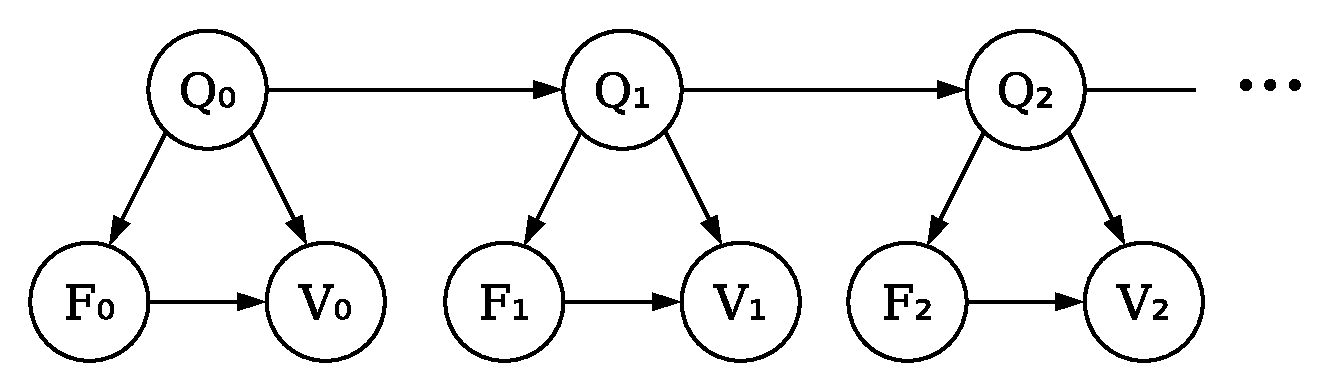
\includegraphics[width=.45\linewidth]{figure/imm}
\caption{Invisible Markov model.}%
\label{fig:imm}
\end{figure}

\newpage
\newpage

\begin{sidewaysfigure}[ht]
    \centering
    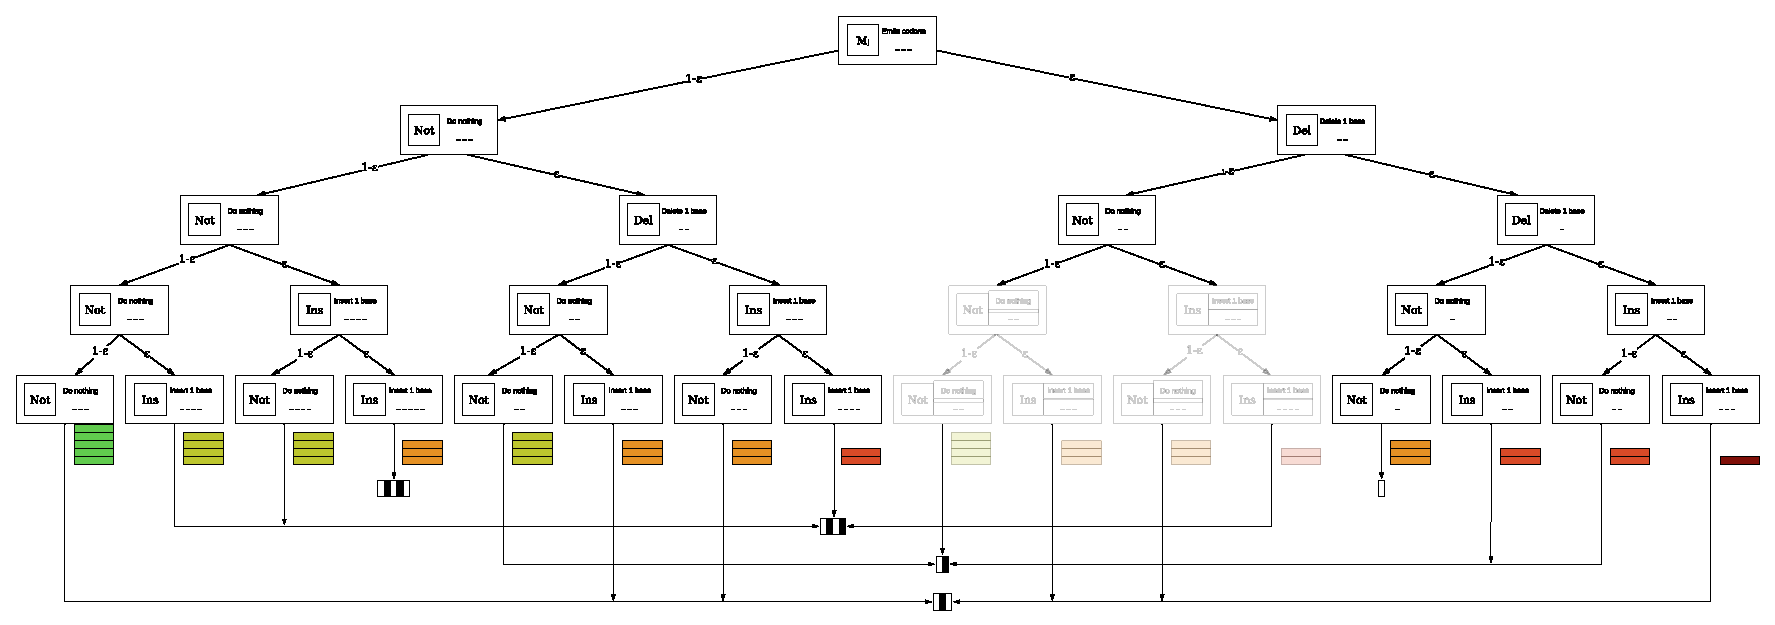
\includegraphics[scale=0.9]{figure/codon-hmm-tree}
    \caption{Matched codon HMM tree.
        The $\eps$-transitions occur infrequently and exist to account for sequence errors.
        The most probably path ends at the first leaf-node from left to right.}\label{fig:codon-hmm-tree}
\end{sidewaysfigure}

% Writting the marginal likelihood as in Eq. \eqref{eq:ml} is rather tedious.
% To alleviate this problem, let $F_t$ be the sequence length emitted by $S_t$,
% $L_t \eqdef 0+F_1+\dots+F_{t-1}$, and $S_{1..t} \eqdef S_1||S_2||\dots||S_t$.
% We have
% \begin{align*}
%   p(S_{1..1} \neq \arr{z}, S_{1..2} \neq \arr{z}, \dots, S_{1..{t-1}} \neq \arr{z}, S_{1..t}=\arr{z})
%   = p(S_{1..t}=\arr{z}, L_t<L).
% \end{align*}
% Therefore, the marginal likelihood is also given by
% \begin{align*}
%   \mathrm{ML}(\arr{z}) = \sum_{t=1}^{\infty} p(S_{1..t}=\arr{z}, L_t<L).
% \end{align*}
